\documentclass[14pt, professionalfont]{article}

\usepackage{amssymb, amsfonts, amsthm}
\usepackage[fleqn]{amsmath}
\usepackage[dvipsnames]{xcolor}
\usepackage[many]{tcolorbox}
\usepackage{fancyhdr}
\usepackage{atbegshi}
\usepackage[hidelinks]{hyperref}
\usepackage{float}
\usepackage[left=0.18\paperwidth, right=0.18\paperwidth, top=0.12\paperheight, bottom=0.18\paperheight]{geometry}


\usepackage{graphicx}
\usepackage{framed}

\usepackage[perpage]{footmisc}
\usepackage{wrapfig}
\usepackage{subcaption}
\usepackage{booktabs}
\usepackage{tabu}

\usepackage{xepersian}
\settextfont{IRLotus}
\setdigitfont{IRLotus}
\setlatintextfont{Neuton}

\renewcommand{\baselinestretch}{1.15} 
\setlength{\mathindent}{0pt}
\setcounter{secnumdepth}{4}
\setcounter{tocdepth}{4}
\hypersetup{
	colorlinks=false,
	pdfborder={0 0 0},
}

\title{ پروژه ۱ سیستم های مخابرات 
	}
\author{دکتر صباغیان}
\date{نیم سال اول 98-99 }

\makeatletter
\let\thetitle\@title
\let\theauthor\@author
\let\thedate\@date
\makeatother

\pagestyle{fancy}
\fancyhf{}
\rhead{\theauthor}
\lhead{\thetitle}
\cfoot{\thepage}

\newcommand{\E}{\text{$\mathbb{E}$}}
\renewcommand{\P}{\text{$\mathbb{P}$}}

\begin{document}	
	\begin{titlepage}
		\centering
		\vspace*{2 cm}
		\begin{minipage}{\textwidth}
			\begin{minipage}{0.5\textwidth}
				\flushright
				
\includegraphics[scale = 0.55]{ece.png}
				\vspace*{0.5 cm}
			\end{minipage}
			\begin{minipage}{0.5\textwidth}
				\flushleft
				
\includegraphics[scale = 0.30]{ut.png}
				\vspace*{0.5 cm}
			\end{minipage}		
		\end{minipage}
	
		\textsc{\LARGE دانشکده فنی دانشگاه تهران}\\[0.5 cm]
		\textsc{\Large دانشکده برق و کامپیوتر}\\[0.5 cm]
		\rule{\linewidth}{0.2 mm}
		{ \LARGE  \bfseries \vspace{5pt} \thetitle}\\
		\vspace{5 pt}
		{\LARGE
			\lr{fourier transform, correlation and energy spectral density}}
		
		\rule{\linewidth}{0.2 mm} \\[1.5 cm]
		\begin{minipage}{0.2\textwidth}
			\begin{flushright} \large
				\emph{طراح:}\\
				\rl{سجاد پاکدامن ساوجی}
				
			\end{flushright}
		\end{minipage}~
		\begin{minipage}{0.3\textwidth}
			\begin{flushleft} \large
				\emph{رایانامه} \\
				\lr{sj.pakdaman@ut.ac.ir}
			\end{flushleft}
		\end{minipage}\\[2 cm]
		{\large \thedate}\\[2 cm]
		\vfill
	\end{titlepage}
{ \Large
	
	دانشجویان عزیز، قبل از پاسخ‌گوئی به سوالات به نکات زیر توجه کنید:
	\begin{enumerate}
	\item 
	شما باید کدها و گزارش خود را با الگو
	\:
	\lr{CA1\_StudentNumber.zip}
	\:
	در محل تعیین شده آپلود کنید
	\item 
	گزارش کار شما معیار اصلی ارزیابی خواهد بود در نتیجه زمان کافی	 برای تکمیل آن اختصاص دهید
	\item 
	
	قسمت اصلی کد شما باید در محیط 
	\:
	\lr{matlab live editor}
	\:
	نوشته شود و نمودار ها علاوه‌ بر گزارش کار باید در کد اصلی نیز قرار داشته باشند
	\item
	توصیه می‌شود پیش‌ از شروع به انجام تمرین قسمت یادآوری روابط را در صفحه ۳ مطالعه کنید
	\item 
	شما میتوانید سوالات خود را از طریق ایمیل
	\textcolor{blue}{
		\: 
		\href{mailto:sj.pakdaman@ut.ac.ir}{sj.pakdaman@ut.ac.ir}
		\:}
	بپرسید
	\end{enumerate}
}
	
	\thispagestyle{empty}
	\clearpage
	\pagenumbering{arabic} 
	\pagebreak
	
	در این تمرین کامپیوتری به پیاده‌سازی  و بررسی روابط ریاضی مباحث 
	\:
	سیگنال و سیستم 
	\:
	و هم بستگی سیگنال های غیر احتمالاتی می‌پردازیم و در انتها، صحت رابطه ی هم بستگی و انرژی ورودی-خروجی سیستم های خطی تغییر نا پذیر با زمان را می سنجیم.
	
	
	\begin{enumerate}
	\item
	فایل صوتی بارگذاری شده را با استفاده از تابع
	\:
	\lr{audioread()}
	\:
	 در متلب بخوانید.(دقت کنید که فرکانس نمونه‌برداری را نیز از تابع خروجی بگیرید) می‌توانید صوت را با استفاده از تابع
	\:
	\lr{sound()}
	\:
	پخش کنید. با استفاده از تابع 
	\:
	\lr{fft()}
	\:
	 اندازه و فاز تبدیل فوریه صوت را بر حسب 
	\:
	\lr{Hz}
	\:
	رسم نمایید.
		\begin{figure}[h]
		\centering
		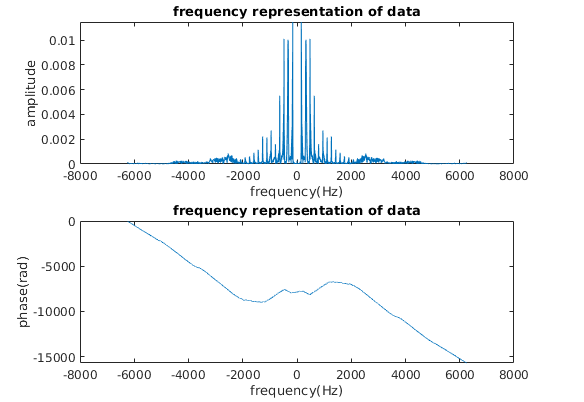
\includegraphics[scale = 0.30]{../images/fourier_of_sound.png}
		\caption{اندازه و فاز تبدیل فوریه صوت}
		\end{figure}
	\item 
	هم‌بستگی بین دو سیگنال از دو روش مستقیم و مبنی بر کانولوشن قابل محاسبه است. برای هر یک از روش ها تابعی پیاده سازی کنید و با مقایسه خروجی توابع اعمال شده بر صوت قسمت قبل ، یکسانی  عملکرد دو تابع را بسنجید.(خروجی دو تابع را رسم کنید)
	
	در روش مستقیم می‌توانید از تابع 
	\:
	\lr{dsp.Crosscorrelator}
	\:
	 و برای انجام کانولوشن می‌توانید از تابع
	\:
	\lr{conv()}
	\:
	استفاده کنید. توجه داشته باشید که توابع فوق در محیط گسسته پیاده سازی شده‌اند بنابر‌این برای تطبیق نتایج با محیط پیوسته باید مقادیر خروجی را باضریب مناسب اسکیل کنید. دلیل انتخاب این ضریب را توضیح دهید.
	
	\item 
	سیگنال شکل ۲ را در نظر بگیرید. سیگنال را ،با فرکانس نمونه‌برداری مناسب، نمونه برداری کنید و با‌استفاده از یکی از توابع قسمت ۲ ، تابع هم‌بستگی سیگنال را رسم نمایید. از روی سیگنال 
	$x(t)$
	سیگنال 	
	$y(t)$
	 را تولید کنید. سیگنال $y(t)$
	  و تابع خودهمبستگی $R_y$ را رسم نمایید و مشاهدات خود را با مفهوم هم‌بستگی توجیح کنید.
	  	$$y(t) = x(t) + 0.7x(t-\frac{1}{4}) + 0.7x(t+\frac{1}{4}) + \frac{1}{3}x(t-\frac{1}{3}) +‌
	  \frac{1}{3}x(t+\frac{1}{3})$$
	  
	  	\begin{figure}[H]
	  	\centering
	  	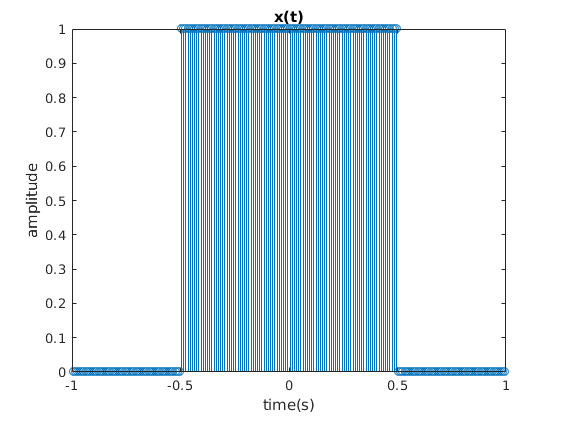
\includegraphics[scale = 0.30]{../images/palse.png}
	  	\caption{
	  		سیگنال
	  		$x(t)$
	  	}
	  \end{figure}
  
  
  \item 
  انرژی یک سیگنال از روش‌های مختلفی قابل محاسبه است. انرژی یک سیگنال را می‌توان با انتگرال گیری در زمان ، استفاده از تابع هم‌بستگی در مقدار $0$ و یاانتگرال گیری از چگالی طیف انرژی 
  \:
  \lr{(ESD)}
  \:
  بدست آورد.
  
  $\bullet$\:
  انرژی سیگنال 
  $x(t)$
  را با استفاده از رابطه حوزه زمان بدست آورید.
  
  $\bullet$\:
  انرژی سیگنال 
  $x(t)$
  را با استفاده از تابع هم‌بستگی 
  $R_x(0)$
  بدست آورید.
  
  $\bullet$\:
  تابع چگالی طیف انرژی سیگنال را ابتدا با اعمال تبدیل فوریه بر تابع هم‌بستگی 
  $R_x$
  و سپس با مجذور تبدیل فوریه سیگنال 
  $x(t)$
  بدست آورید و آن ها‌را رسم نمایید. با محاسبه سطح زیر نمودار این توابع انرژی سیگنال 
  $x(t)$
  برای هر دو روش محاسبه کنید. بدیهی است که انرژی بدست آمده از روش های متفاوت باید یکسان باشد. 
  
    \item 
    فیلتر 
    $h(t)$ 
    شکل ۳ را در‌نظر بگیرید. تابع هم‌بستگی و چگالی طیف انرژی این فیلتر را رسم کنید. (
    $h(t)$
    و
    $x(t)$
    باید فرکانس نمونه برداری یکسانی داشته باشند
    )
    
    فیلتر 
    $h(t)$ 
    را با استفاده از 
    \:
    \lr{conv()}
    \:
     بر سیگنال
   $x(t)$
    اعمال کنید و تابع هم‌بستگی و چگالی طیف انرژی خروجی را رسم نمایید.
    
    در ادامه میخواهیم درستی رابطه بین توابع هم‌بستگی ورودی-خروجی فیلتر(۱) و رابطه بین انرژی ورودی-خروجی فیلتر(۲) را بسنجیم. برای هر رابطه دو طرف تساوی را جداگانه محاسبه و رسم نمایید و یکسانی طرفین را بررسی کنید.
    
   
\begin{figure}[h]
	\begin{subfigure}{.5\textwidth}
		\centering
		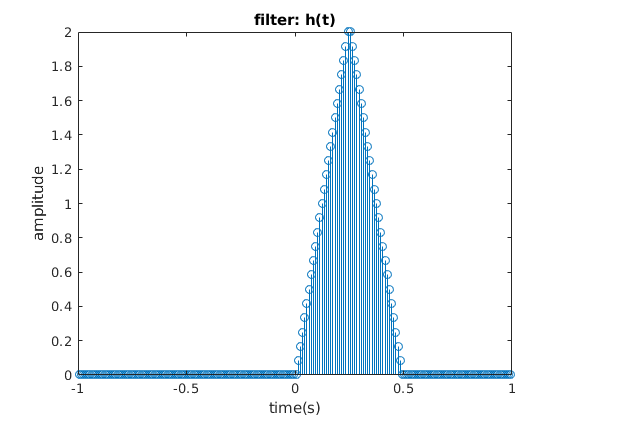
\includegraphics[scale = 0.30]{../images/filter.png}
		\caption{
			فیلتر
			$h(t)$
		}
	\end{subfigure}%
	\begin{subfigure}{.5\textwidth}
		\centering
		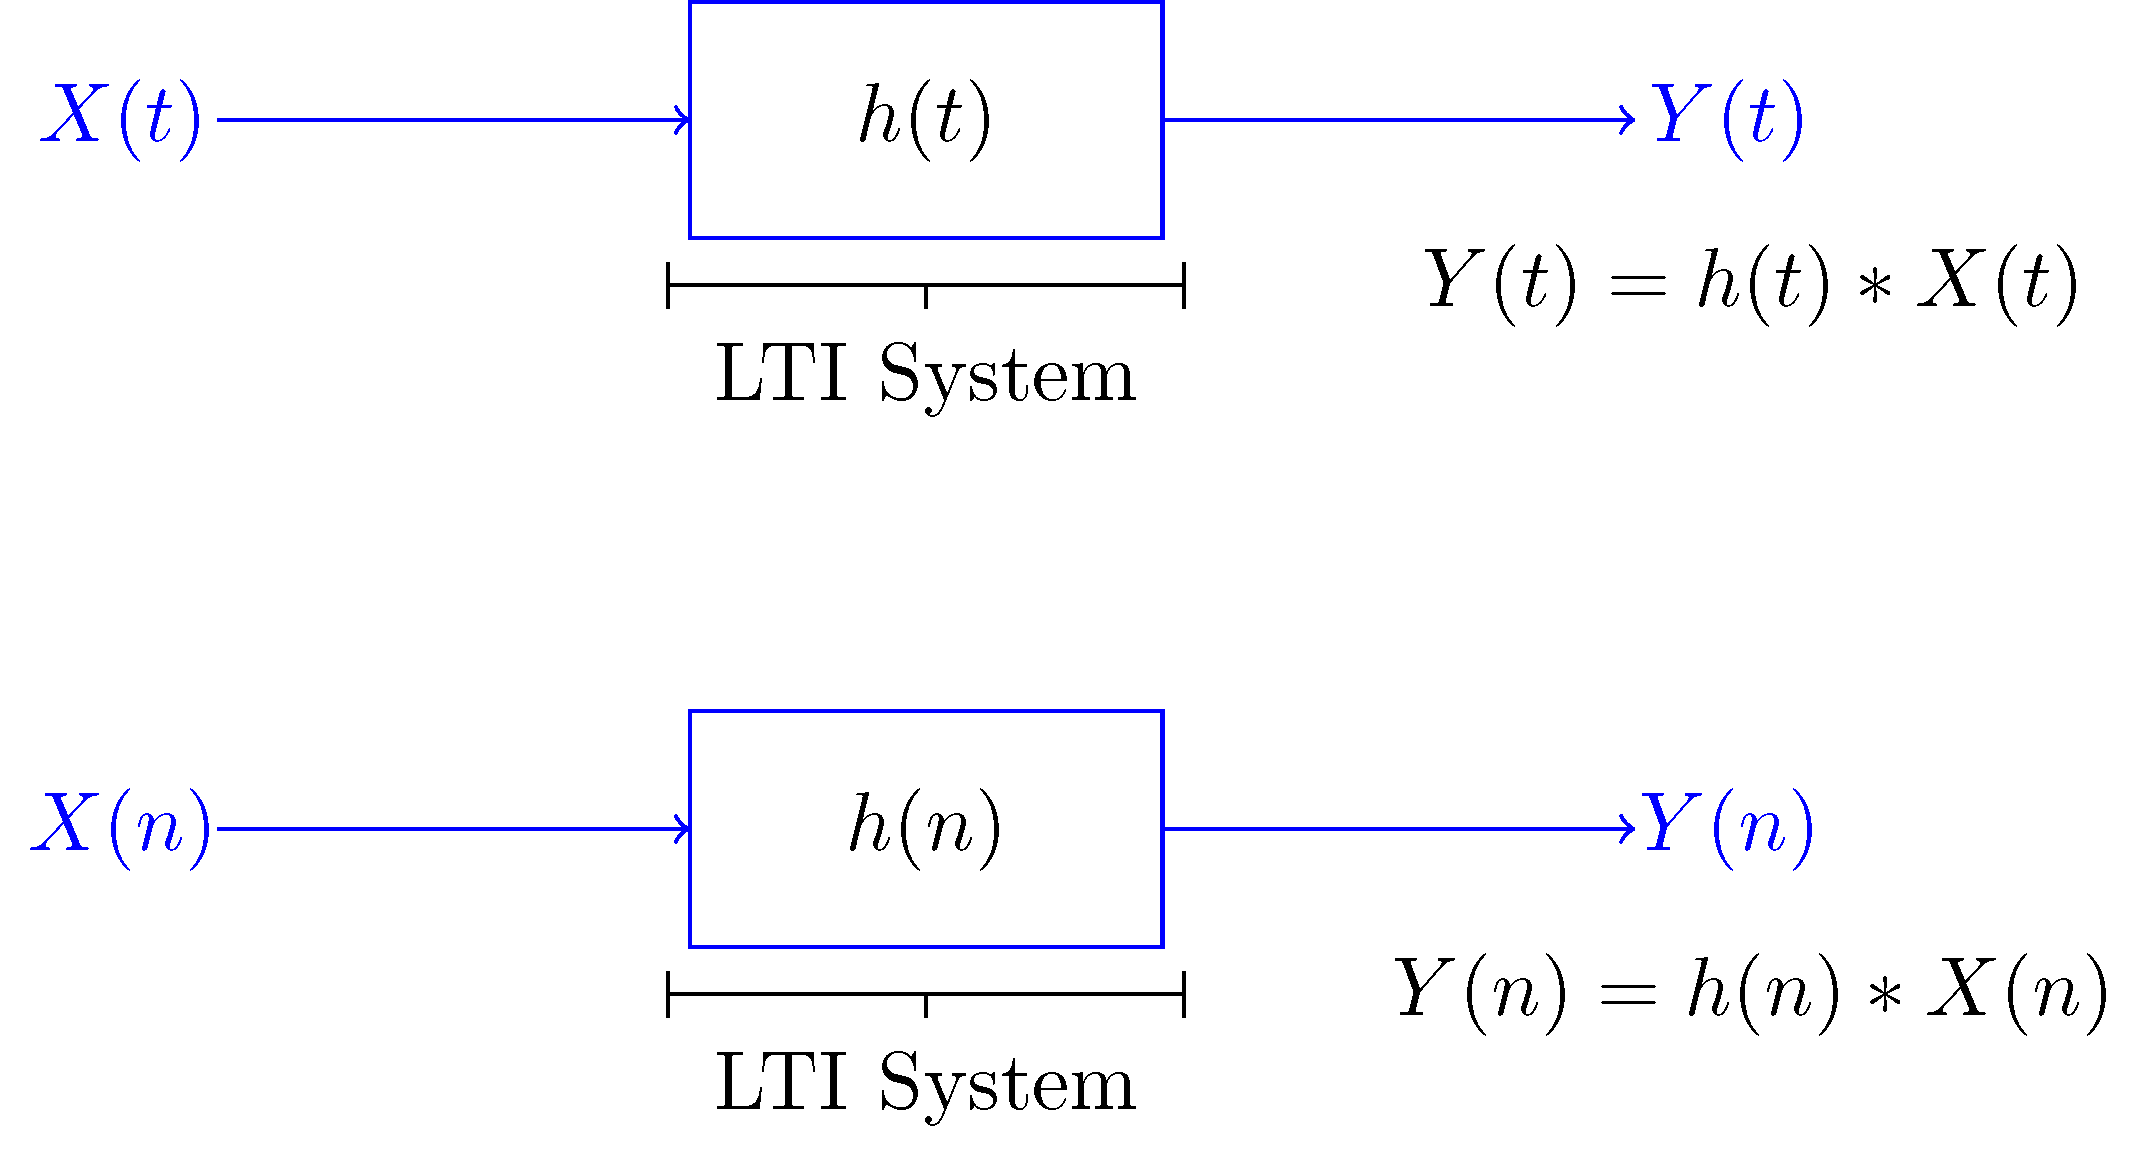
\includegraphics[scale = 0.70]{../images/lti.png}
		\caption{
			\lr{LTI system}
		}
	\end{subfigure}
	\caption{ }
	\label{fig:fig}
\end{figure}

 \begin{equation}
R_y(\tau) = R_x(\tau)*h(\tau)*h^*(-\tau)
\end{equation} 
\begin{equation}
S_y(f) = S_x(f)\times H(f)\times H^*(f)
\end{equation}

	\end{enumerate}
\newpage
\begin{center}
	\textbf{\textit{{\LARGE یادآوری روابط}}}
\end{center}
\flushleft{\lr{energy signal : $E_x = \int_{-\infty}^{\infty}$ $\left|x(t)\right|^2\:dt \; < \infty$\\
power signal : $P_x =\frac{1}{2T}_{T \rightarrow \infty}\int_{-T}^{T}$ $\left|x(t)\right|^2\:dt \; < \infty $}

\vspace{10pt}
$\left<x(t),y(t)\right>  = \begin{cases}
\int_{-\infty}^{\infty} x(t)y^*(t)\: dt \qquad \qquad \qquad energy\: signal\\
\frac{1}{2T}_{T \rightarrow \infty}\int_{-T}^{T} x(t)y^*(t)\: dt \qquad \quad power\: signal\\
\end{cases}$
\lr{
\begin{equation*}
	||x(t)||^2 = \left<x(t),x(t)\right> = \begin{cases}
	E_x \qquad energy\:signal\\
	P_x \qquad power \: signal\\
	\end{cases}
\end{equation*}
\begin{equation*}
	R_{x,y}(\tau) = \left<x(t),y(t-\tau)\right> \qquad R_{x,y}(\tau) =x(\tau)*y^*(-\tau)
\end{equation*}
\begin{equation*}
	R_x(\tau) = R_{x,x}(\tau) \qquad R_x(0) = \begin{cases}
	E_x \qquad energy\:signal\\
	P_x \qquad power \: signal\\
	\end{cases}
\end{equation*}
Energy Spectrum Density (ESD) is for energy signals
\begin{equation*}
S_x(f) = |X(f)|^2 \qquad \int_{-\infty}^{\infty} |X(f)|^2 \: df = \int_{-\infty}^{\infty} |x(t)|^2 \: dt \quad Parseval's \:theorem
\end{equation*}
Power Spectrum Density (PSD) is for power signals
\begin{equation*}
S_x(f) = \lim_{T\rightarrow \infty} \frac{|X_T(f)|^2}{2T} \qquad X_T(f)  =F\left\{x_T(t)\right\} \qquad x_T(t)= \begin{cases}
x(t) \quad |t|<|T| \\
0 \qquad \; o.w
\end{cases}
\end{equation*}
}
}
\end{document}